\documentclass[letterpaper]{article}
\usepackage{amssymb}
\usepackage{fullpage}
\usepackage{changepage}
\usepackage{amsmath}
\usepackage{amsthm}
\usepackage{amsfonts}
\usepackage{epsfig,float,alltt}
\usepackage{psfrag,xr}
\usepackage[T1]{fontenc}
\usepackage{url}
\usepackage{pdfpages}
\usepackage{epstopdf}
\usepackage[framed,numbered,autolinebreaks,useliterate]{mcode}

%\includepdfset{pagecommand=\thispagestyle{fancy}}
\author{Fan Bu, Feng Zhou, Yi Yang}
\title{ME 552 Lab 02B Report}

\begin{document}
\date{09/04/2016}
\maketitle

\newcommand{\trace}{\mathrm{trace}}
\newcommand{\real}{\mathbb R}  % real numbers  {I\!\!R}
\newcommand{\nat}{\mathbb N}   % Natural numbers {I\!\!N}
\newcommand{\cp}{\mathbb C}    % complex numbers  {I\!\!\!\!C}
\newcommand{\ds}{\displaystyle}
\newcommand{\mf}[2]{\frac{\ds #1}{\ds #2}}
\newcommand{\spanof}[1]{\textrm{span} \{ #1 \}}
\newcommand{\sol}[0]{\textbf{Solution: }}
\newcommand{\pf}[0]{\textbf{Proof:}}
\newcommand{\rme}[0]{\textrm{e}}
\newcommand{\Null}[1]{\textrm{Null}\{#1\}}
\parindent 0pt
%%%%%%%%%%%%%%%%%%%%%%%%%%%%%%%%%%%%%%%%%%%%%%%%%%%%%%%%%%%%%%%%%%%%%%%%%%%%%%%
% Solution for Question 1 begins here - by Yi Yang
%%%%%%%%%%%%%%%%%%%%%%%%%%%%%%%%%%%%%%%%%%%%%%%%%%%%%%%%%%%%%%%%%%%%%%%%%%%%%%%
\section*{Question 1}
\subsection*{(a)}
The overall physical Maglev system can be shown below:
\begin{figure}[H]
	\centering
	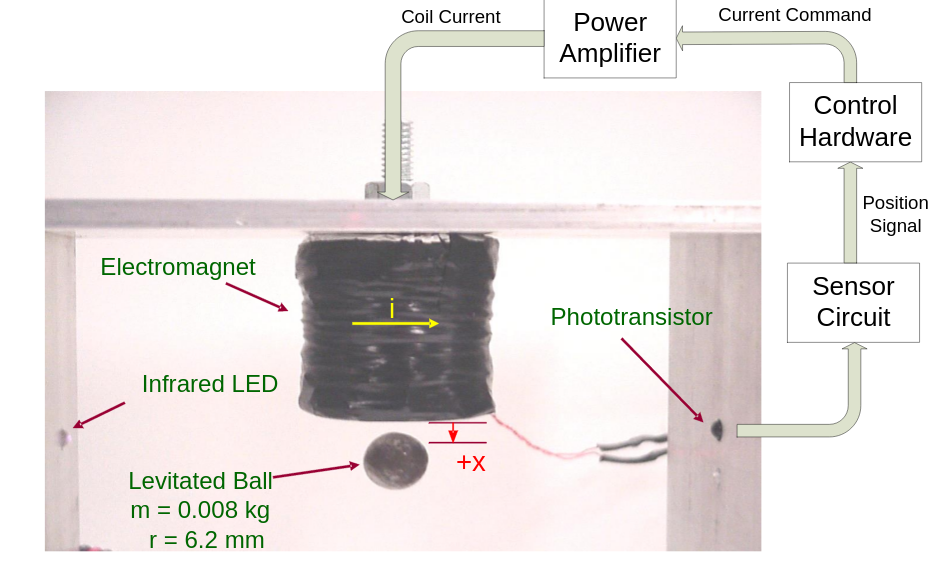
\includegraphics[scale=0.3]{Maglev.png}
	\caption{Physical Maglev System}
\end{figure}
We will divide the overall system into four parts: Feedback Sensor, Driver Circuits, Electromagnet, and Magnet $\&$ Ball system.\\

\textbf{\large{Feedback Sensor}}\\
Assumptions:
\begin{itemize}
	\item The radiation rays are parallel to each other
	\item Neglect light reflected by irrelevant objects in the neighbourhood
	\item Suppose the the cross section of radiation rays is perfect circle and the steel ball is perfect sphere
	\item No other light source in the room interferes the light receptance of photo transistor.
\end{itemize}
Based on the assumptions above, the geometrical relations can drawn from the following picture. We will use $r_1$ and $r_2$ denote the ratios of ball and beam respectively, $d_1$ and $d_2$ represents the distance from center of two circles to the center dash line if the two circles will intersect. The fraction of light received by the sensor then will be represented as a piecewise function $LF$.
\begin{figure}[H]
\centering
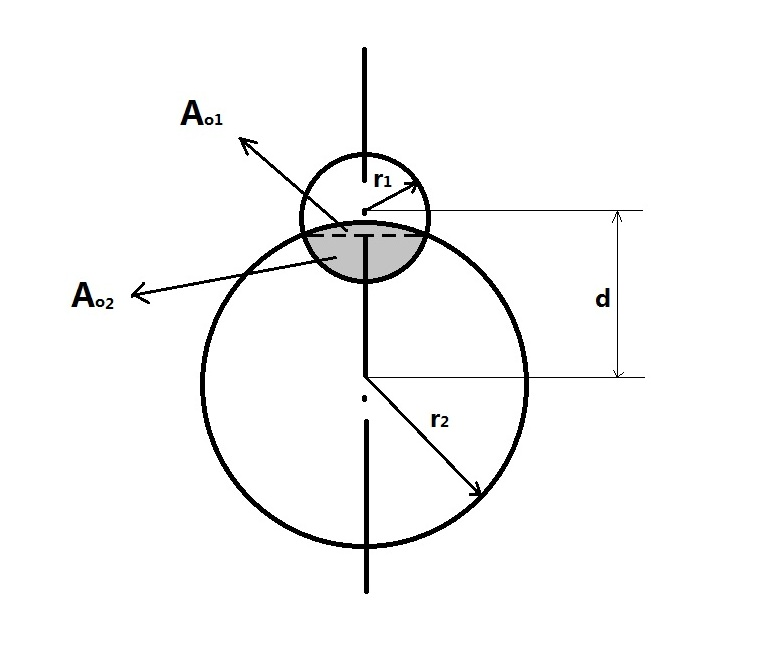
\includegraphics[scale=0.5]{beam.jpeg}
\caption{Sketch of Cross Section of Beam Rays and Ball}
\end{figure} 
\[
   LF = \left\{
  \begin{array}{l l}
    \frac{A_{2} - A_{1}}{A_{2}} & \quad \text{if } r_{1} + |d| < r_{2} \\
    0 & \quad \text{if } r_{2} + |d| < r_{1} \\
    1 & \quad \text{if } |d| > r_{2} + r_{1} \\
    \frac{A_{2} - A_{o}}{A_{2}} & \quad \text{if } |d| < r_{1} + r_{2} \\
  \end{array} \right.
\]
Then we can deduce the following relations:
$$ A_{2} = \pi r_{2}^2$$
$$A_{1} = \pi r_{1}^2 $$ 
$$ y = \frac{d^2+r_{2}^2-r_{1}^2}{2d}$$
$$ d_{2}=y$$
$$ d_{1}=d-y=\frac{d^2-r_{2}^2+r_{1}^2}{2d} $$
$$ A_{o1} = r_{2}^2 \cos^{-1} (\frac{d_{2}}{r_{2}})-d_{2} \sqrt{r_{2}^2-d_{2}^2}$$ 
$$ A_{o2} = r_{1}^2 \cos^{-1} (\frac{d_{1}}{r_{1}})-d_{1} \sqrt{r_{1}^2-d_{1}^2}$$
$$ A_{o} = A_{o1} + A_{o2} $$

\textbf{\large{Driver Circuits}}\\
Assumptions:
\begin{itemize}
	\item voltage at inverting and non-inverting terminals is equal
	\item current at inverting and non-inverting terminals is zero
	\item input impedance is infinite and output impedance is zero
\end{itemize}
The Driver Circuit will be shown as below:
\begin{figure}[H]
	\centering
	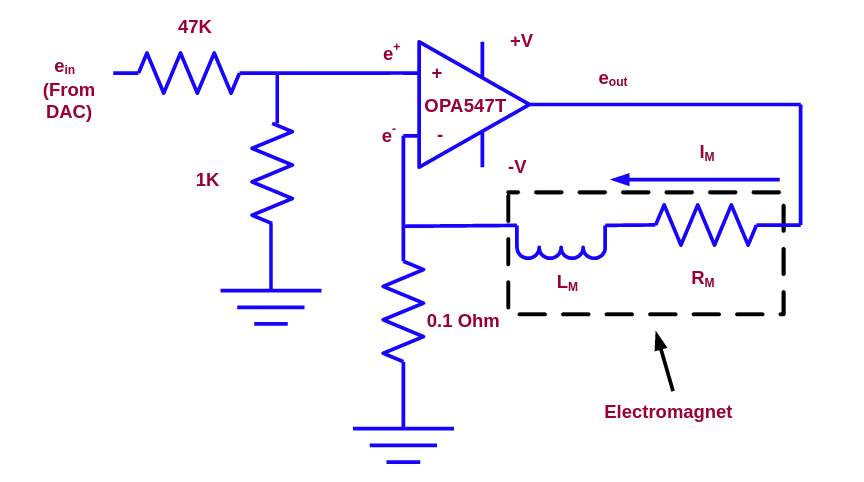
\includegraphics[scale=0.4]{current_driver_circuit.png}
	\caption{Current Driver Circuit}
\end{figure}
We will denote resistance $47K\Omega$, $1K\Omega$ and $0.1\Omega$ as $R_1$, $R_2$ and $R_3$ if the numerical values are not set to them. Then we have:
$$ V^{+}=\frac{R_2}{R_1+R_2}V_{in} \hspace{1cm} I_{EM}=\frac{V^{+}}{R_3}=\frac{1}{R_3}\left(\frac{R_2}{R_1+R_2}\right)V_{in} = DV_{in}$$

\textbf{\large{Electromagnet}}\\
Assumptions:
\begin{itemize}
	\item We use $\mu_{Al}$, $\mu_{Cu}$, $\mu_s$ and $\mu_0$ represents the absolute magnetic permeability of Al, Cu, steel and air respectively and we assume $\mu_{Cu}=\mu_{Al}=\mu_{0}$ and $\mu_s \gg \mu_0$
	\item The steel ball will be modelled as a cylinder with its axis collinear with the electromagnet and the section area in the relative path has relations: $A_{cd} \approx A_{s} = \pi  r_{s}^2 $
	\item We can neglect the effects of fringing on the cross-sectional area of paths through the air and assume particular dimensions that are consistent with the solid objects in the system \\
$$ A_{EM} = \pi r_{EM}^2 \approx A_{ab} \hspace{1cm} A_{s} \approx A_{bc} \approx A_{de} \hspace{1cm} A_{EM} \approx A_{be} + A_{bc} $$ 
	\item Path length from b to c (see figure \ref{fig:Q1_a2}) assumes to be constant
	\item The ball remains in line with the axis of the electro magnet and in front of the magnet $( x > 0 )$
\end{itemize}
The sketch for physical magnet system and simplified circuit are shown below:
\begin{figure}[H]
	\centering
	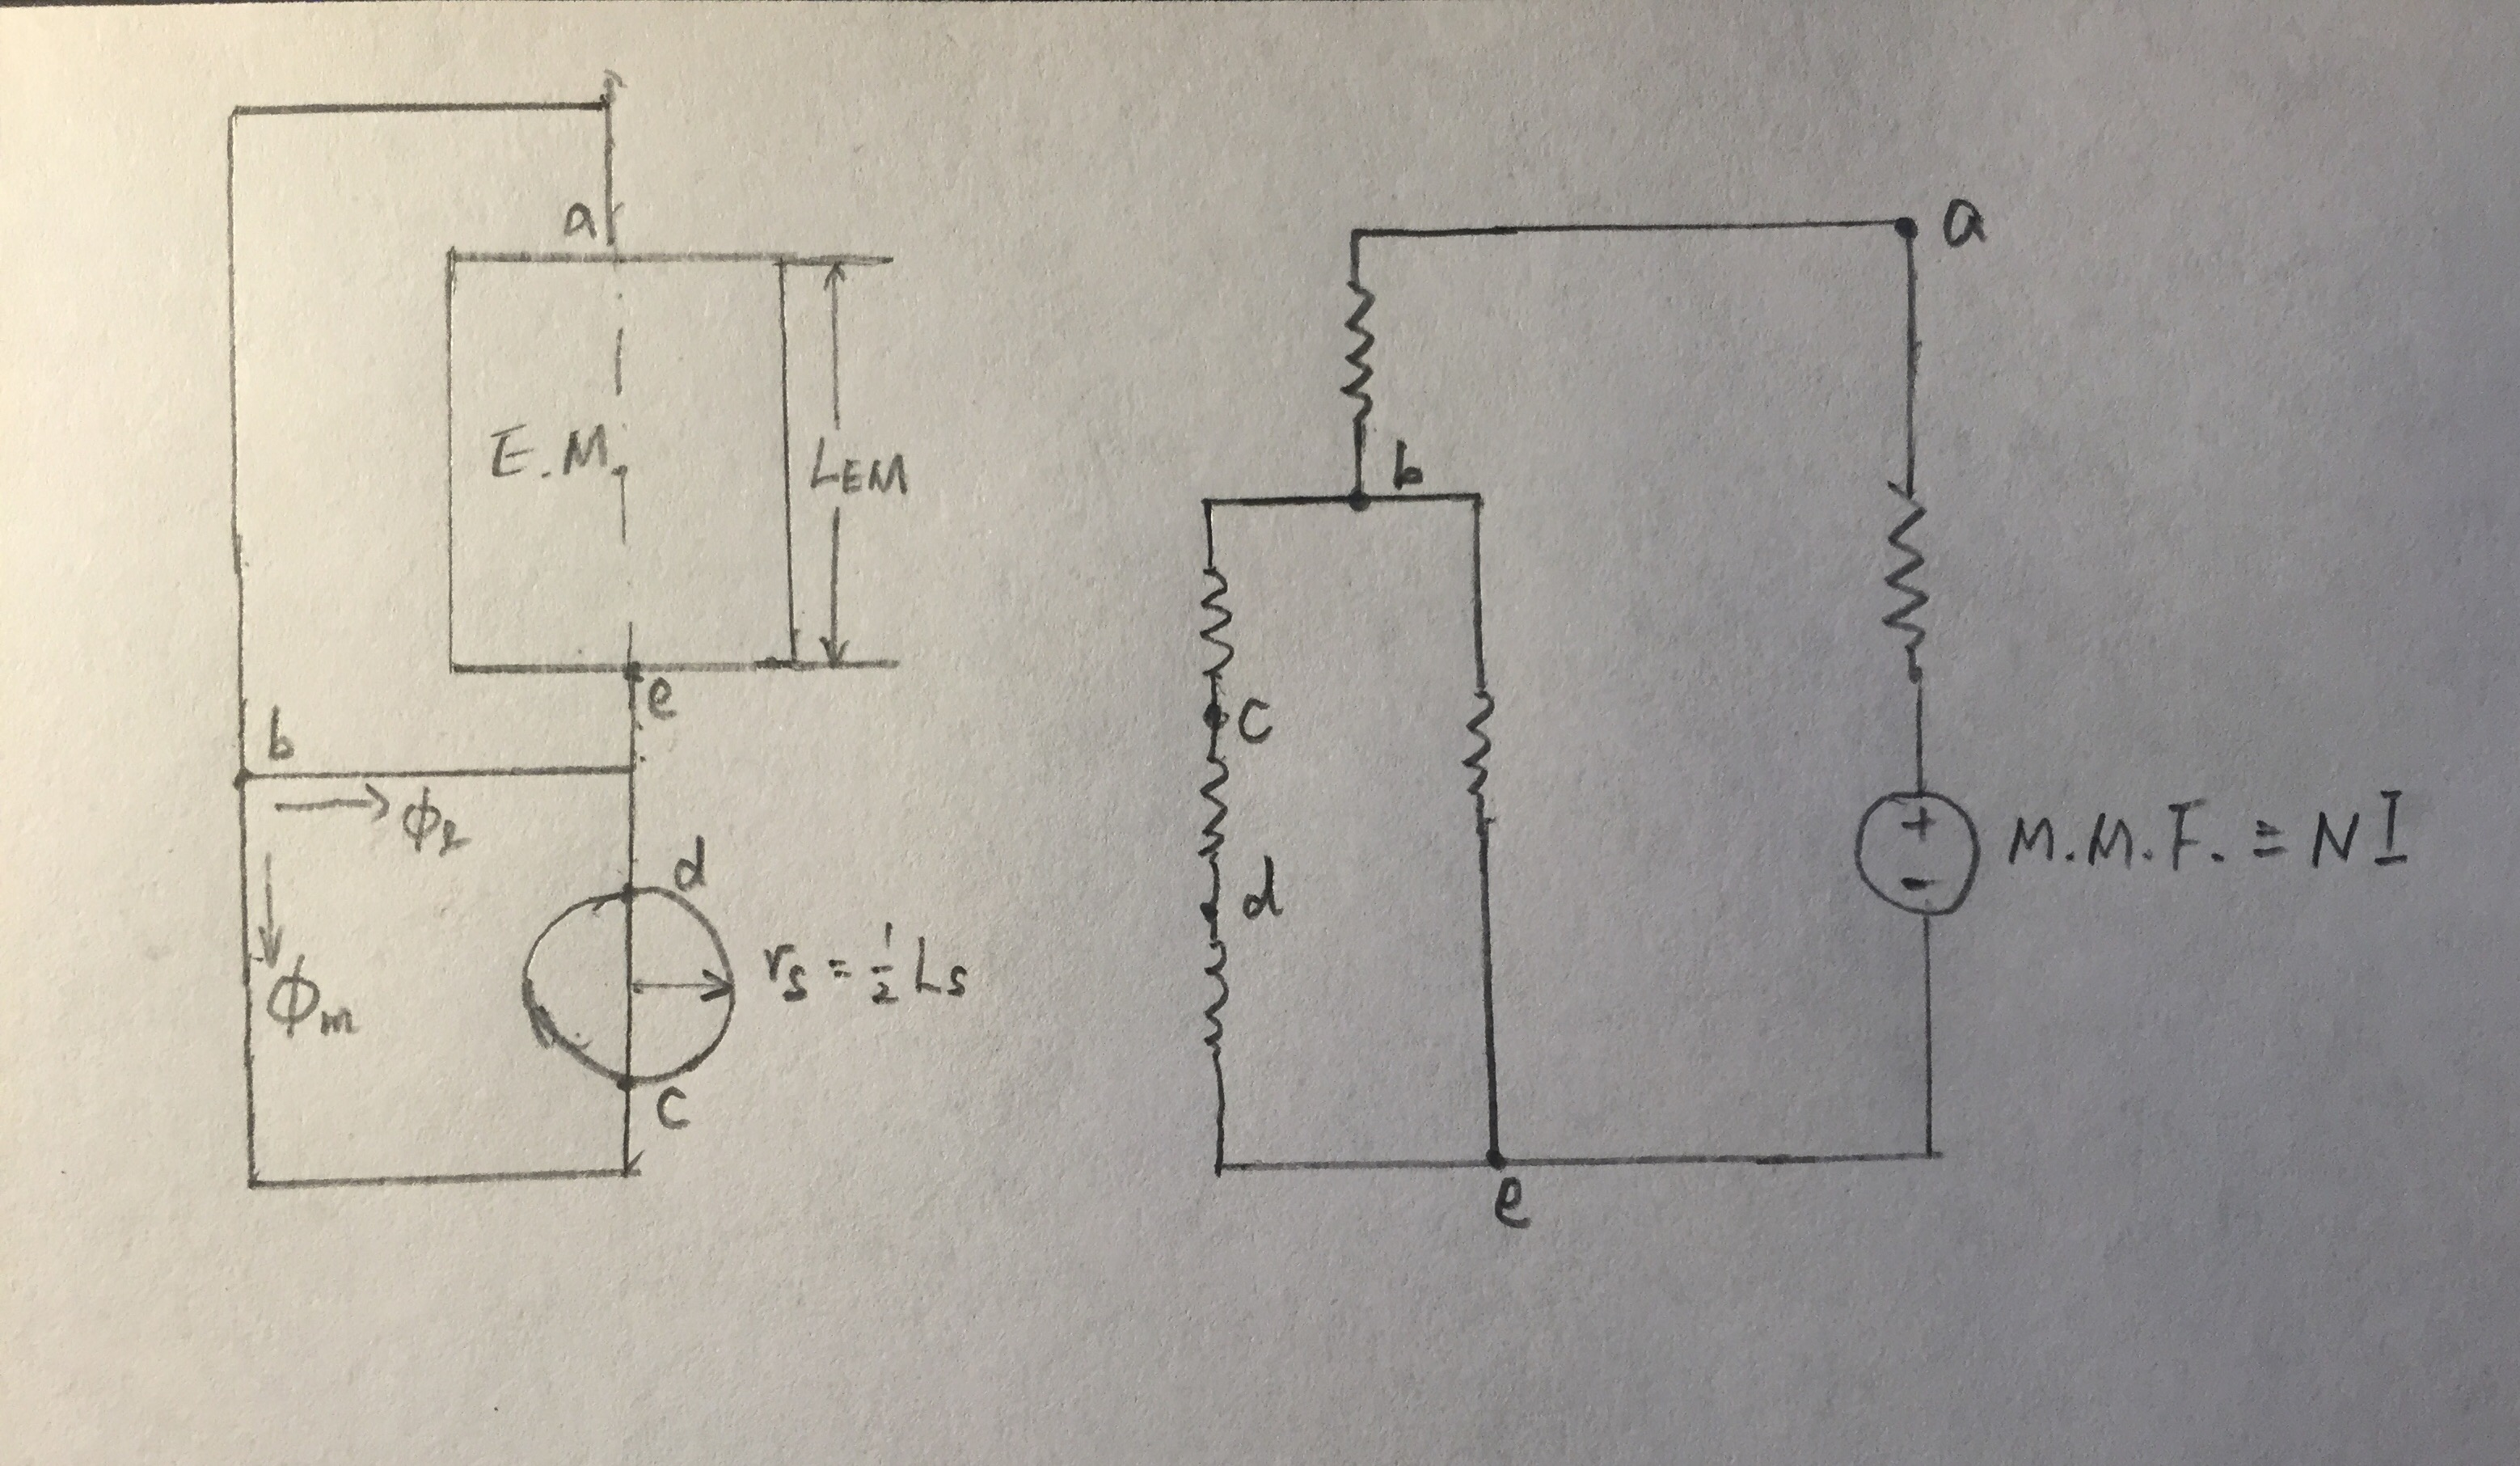
\includegraphics[scale=0.1]{magnet.jpeg}
	\caption{Magnet System and Equivalent Circuit}
	\label{fig:Q1_a2}
\end{figure}
Based on the equivalent circuit, $R_{em}$, $R_{ab}$, $R_{bc}$, $R_{cd}$, $R_{de}$ and $R_{be}$ will represent different parts of magneto impedance of electromagnet system. They will be computed as follows:
$$ R_{em} = \frac{L_{em}}{A_{EM}\mu_{0}}  \hspace{1cm} R_{ab} = \frac{L_{ab}}{A_{em}\mu_{0}} \hspace{1cm} R_{bc} = \frac{L_{bc}}{(A_{s})\mu_{0}} \hspace{1cm} R_{de} = \frac{x}{A_{s}\mu_{0}} \hspace{1cm} $$ $$ R_{be} = \frac{L_{be}}{(A_{em} - A_{s})\mu_{0}}  \hspace{1cm}  R_{s} = \frac{2r_{s}}{A_{s}\mu_{s}} \approx 0$$
We will use Ampere$\prime$s Law to get the relations between magneto motive force and magnetic flux. (Note: we will use subscript $em$ to replace $EM$) Ampere$\prime$s Law:
$$\oint_L \vec{H}\cdot d\vec{L} = i_{enc}$$
Then,
$$ NI = \phi \left (R_{em} + R_{ab}\right) + \phi_{m} \left( R_{bc}+R_{s}+R_{dc} \right) $$
$$ NI = \phi \left( R_{em} + R_{ab} \right) + \phi_{l} \left( R_{be} \right) $$
$$ \phi = \phi_{m} + \phi_{l} $$

Solving the $2^{nd}$ equation for $\phi_{l}$ gives:

$$\phi_{l} = C_{0}\left( NI-C_{1}\phi_{m} \right)$$ 
$$C_{0} = \frac{\mu_{0} A_{em} (A_{em} - A_{s})}{L_{be} A_{em} + (L_{em} + L_{ab})(A_{em} - A_{s}))} \hspace{1cm} 
C_{1} = \frac{L_{em} + L_{ab}}{\mu_{0} A_{em}} $$

Then we can get the magnetic flux through the mover:
$$ \phi_{m} = \frac{NI(1-C_{0}C_{1})}{C_{1} - C_{0} C_{1}^2 + \frac{L_{bc}}{\mu_{0} A_{s}} + \frac{x}{\mu_{0} A_{s}}} $$
Next, we will use self inductance relational formula to calculate the energy stored in the magnetic field and compute the force by taking the derivative of energy function with respect to displacement variable:
$$ \lambda = N \phi = L(x) I $$
$$ W(i,x) = \mf{1}{2} L(x) I^2 = \mf{1}{2} N \phi(x) I =\mf{1}{2} N I (\phi_{m}(x) + \phi_{l}(x))$$
$$ F(i,x) = \mf{d}{dx} (W(i,x) )= \mf{1}{2} N I ( \mf{d}{dx} (\phi_{m}) + \frac{d}{dx} (\phi_{l})) $$

$$ \mf{d}{dx}(\phi_{m}) = - \mf{N I (1 - C_{0}C_{1} \mu_{0} A_{s}}{(\mu_{0} A_{s}(C_{1} - C_{0} C_{1}^2 + C_{2}) + x)^2} dx$$

$$ \mf{d}{dx}(\phi_{l}) = -C_{0} C_{1} \mf{d}{dx}(\phi_{m})$$
Hence, we can get the electromagnetic force:
$$ F_{em}(x) = -\mf{1}{2} \left( 1 - C_{0}C_{1} \right)^2 \mf{\mu_{0} A_{s} N^2 }{(\mu_{0} A_{s}(C_{1} - C_{0} C_{1}^2 + C_{2}) + x)^2} I^2 $$
In order to get the full expression of $F_{em}$, we decide to rewrite the formula above as:
$$ F_{em}(x) = -\frac{A I^2}{(B+x)^2} $$
where $A$, $B$ are parameters to be obtained from identification experiments.\\

\textbf{\large{Magnet \& Ball System}}\\
Assumptions:
\begin{itemize}
	\item Ignore the air resistance
	\item assume the distance between ball and magnet is always positive, denoted as $x$.
\end{itemize}
According to classical Newton$\prime$s $2$nd Law:
$$ \sum F_x = mg + F_{EM} = mg -\frac{A I^2}{(B+x)^2} = m  \ddot{x}$$

%%%%%%%%%%%%%%%%%%%%%%%%%%%%%%%%%%%%%%%%%%%%%%%%%%%%%%%%%%%%%%%%%%%%%%%%%%%%%%%
% Solution for (b) starts here
%%%%%%%%%%%%%%%%%%%%%%%%%%%%%%%%%%%%%%%%%%%%%%%%%%%%%%%%%%%%%%%%%%%%%%%%%%%%%%%
\subsection*{(b)}
\textbf{\large{Feedback Sensor}}\\
In order to linearize the function $LF$ with respect to $x$, we must find the geometric relations between $x$ and $d$. We sketch the figure below:
\begin{figure}[H]
	\centering
	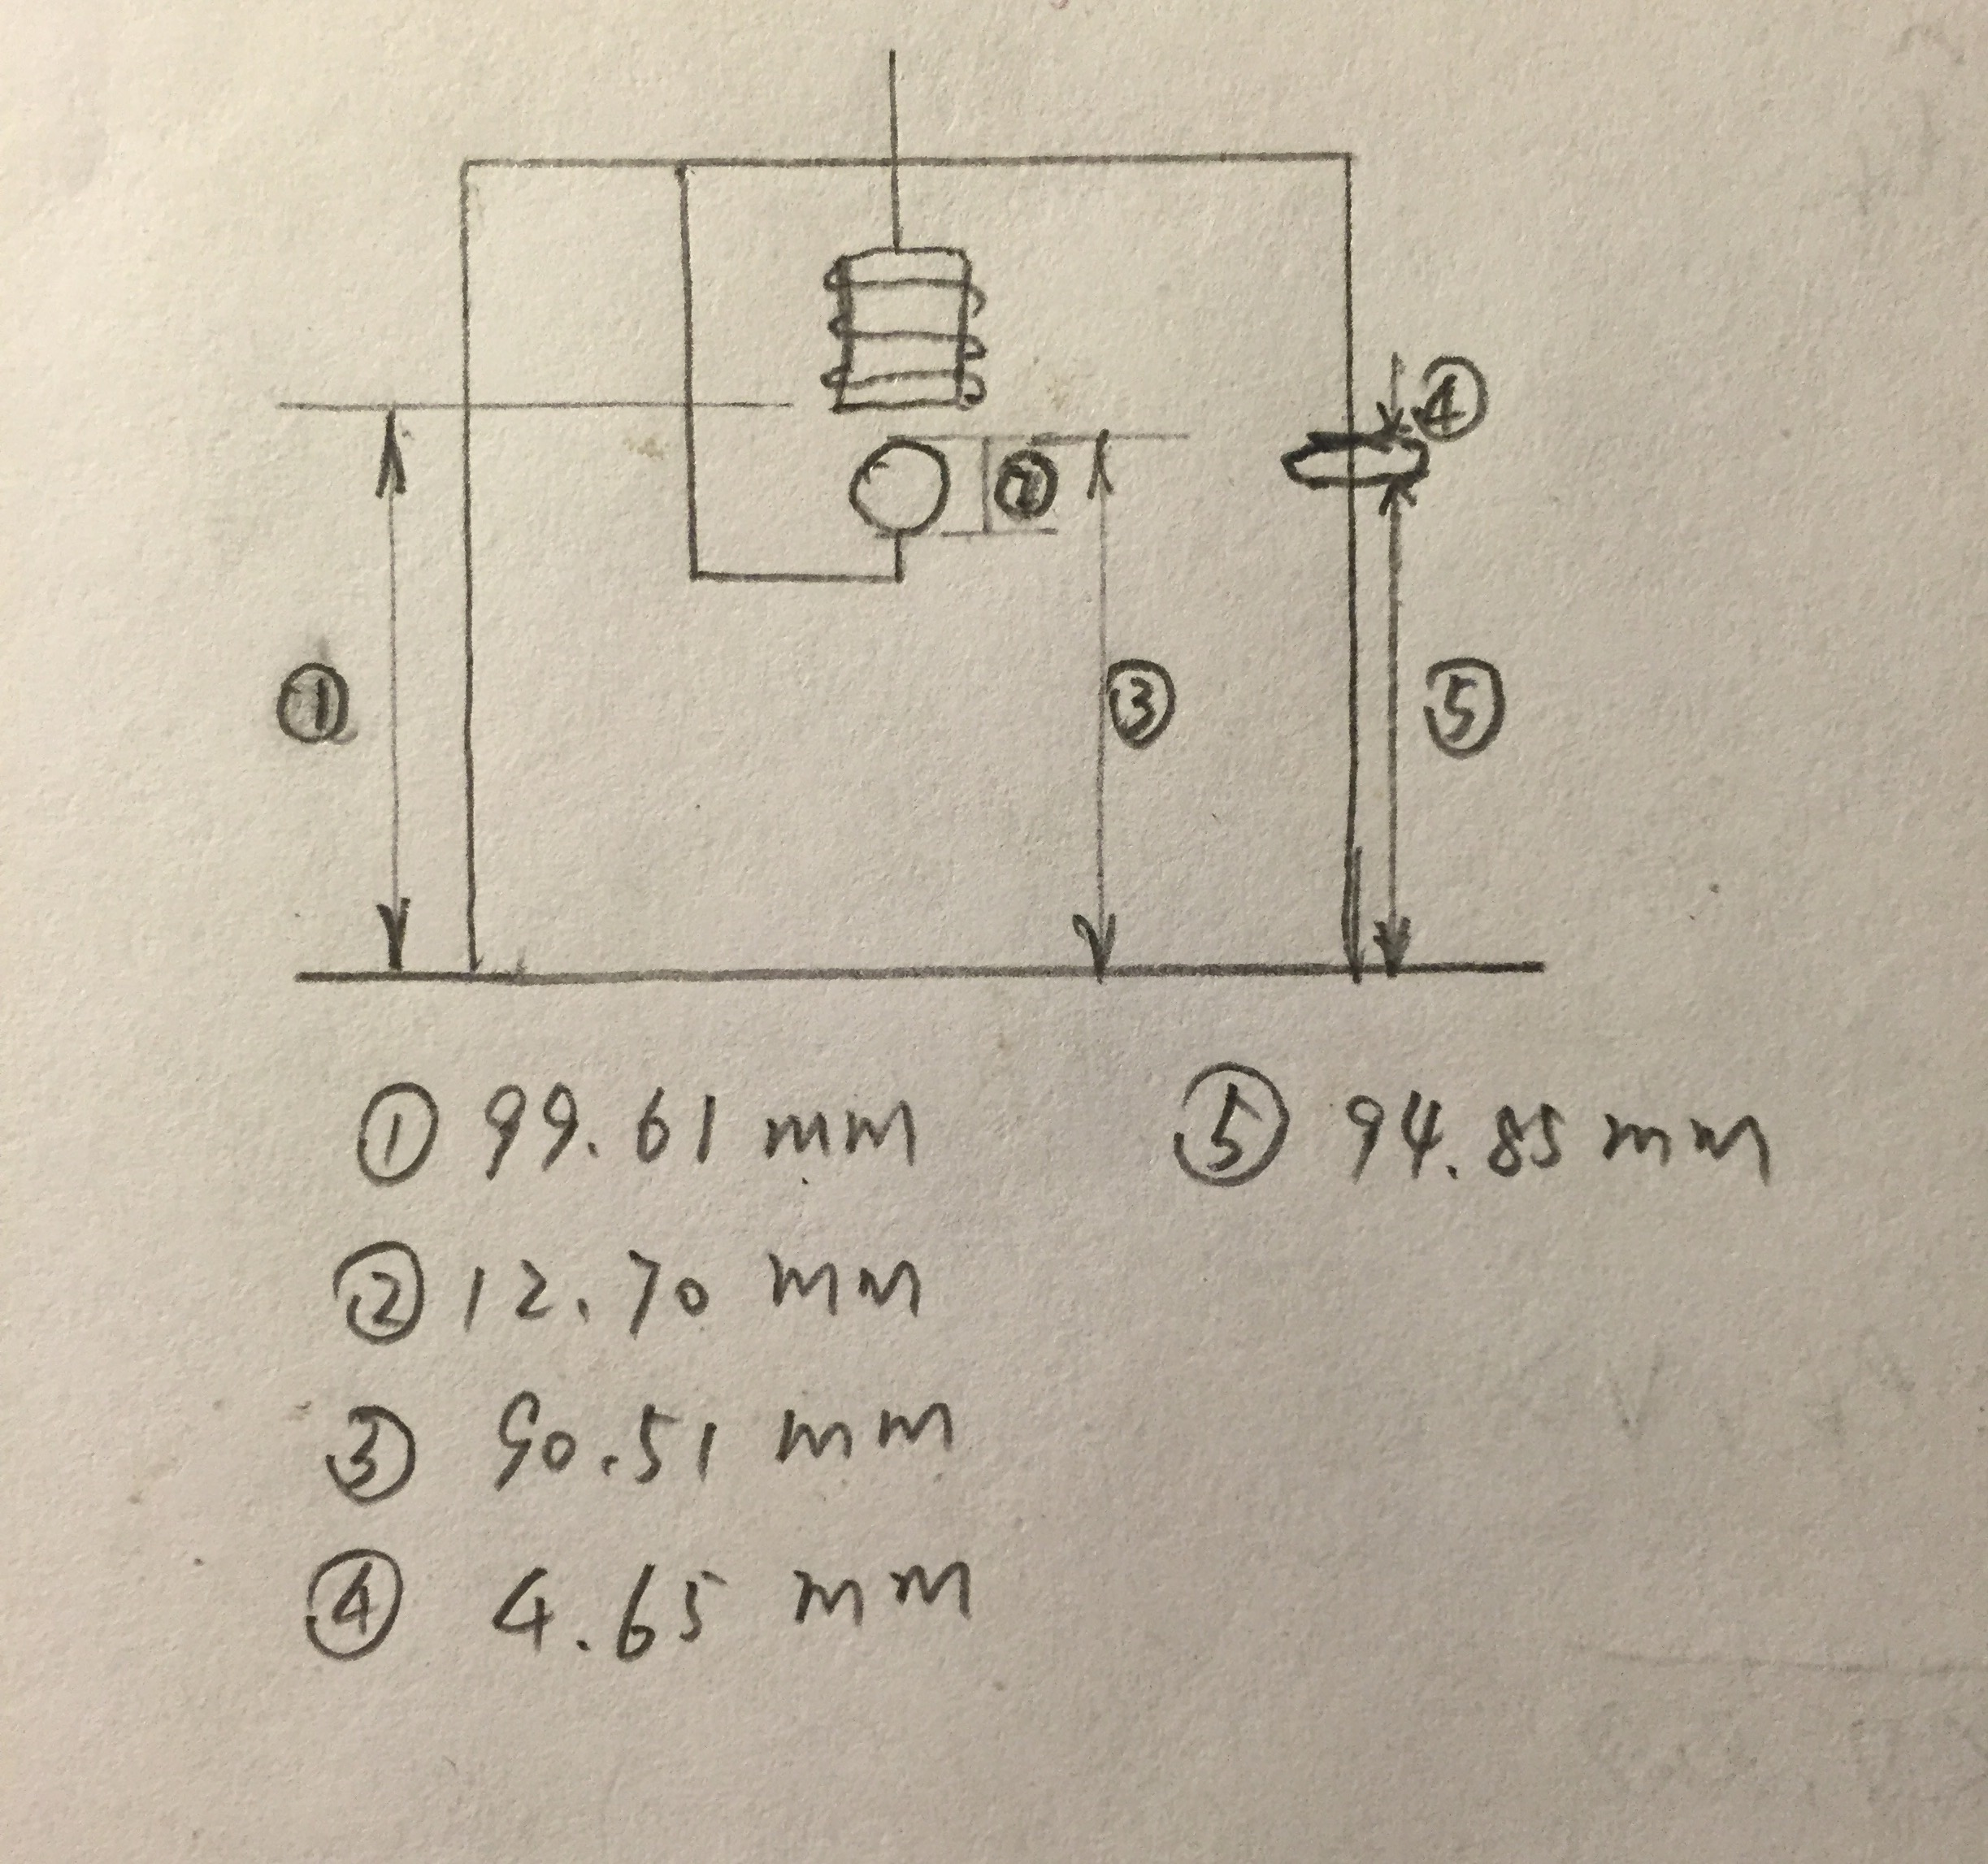
\includegraphics[scale=0.08]{dx_revised.jpeg}
	\caption{Geometric Relations Between Steel Ball and Light Rays}
\end{figure}
The geometric parameters are measured and shown in the graph, we have $h_{magnet} = 99.61$, $r_s = 6.35$, $h_s = 90.51$, $d_{sensor} = 4.65$ and $h_{sensor} = 94.85$, then we have following relations between $x$ and $d$:
$$x = d + h_{magnet}-h_{sensor}-\mf{1}{2}d_{sensor}-r_s=d-3.915$$
First, we need to derive relations between $LF$ and $d$:
$$ A_{o} = A_{o1} + A_{o2} \hspace{1cm}  \frac{\partial A_{o}}{\partial d} = \mf{\partial A_{o1}}{\partial d}  + \mf{\partial A_{o2}}{\partial d} $$
For $A_{o1}$ we have:
$$ A_{o1} = r_{1}^2 \cos^{-1} (\mf{d_{1}}{r_{1}})-d_{1} \sqrt{r_{1}^2-d_{1}^2} $$
$$ \frac{\partial A_{o1}}{\partial d} = \left( -\mf{r_{1}}{\sqrt{1 - \left(\mf{d_{1}}{r_{1}}\right)^2}} - \left( r_{1}^2 - d_{1}^2\right)^{\tfrac{1}{2}} + d_{1}^2 \left( r_{1}^2 - d_{1}^2\right)^{-\tfrac{1}{2}} \right) \frac{\partial d_{1}}{\partial d}$$
The same way we will get relations between $A_{o2}$ and $d$:
$$ A_{o2} = r_{2}^2 \cos^{-1} (\mf{d_{2}}{r_{2}})-d_{2} \sqrt{r_{2}^2-d_{2}^2}$$ 

$$ \mf{\partial A_{o2}}{\partial d} = \left( -\mf{r_{2}}{\sqrt{1 - \left(\mf{d_{2}}{r_{2}}\right)^2}} - \left( r_{2}^2 - d_{2}^2\right)^{\tfrac{1}{2}} + d_{2}^2 \left( r_{2}^2 - d_{2}^2\right)^{-\tfrac{1}{2}} \right) \mf{\partial d_{2}}{\partial d}$$
We also need to find $\tfrac{\partial d_1}{\partial d}$ and $\tfrac{\partial d_2}{\partial d}$:
$$ d_{2}=y \hspace{1cm} \mf{\partial d_2}{\partial d} =  \frac{\partial y}{\partial d} = \left(\mf{1}{2}  -\mf{r_{2}^2}{2d^2} + \mf{r_{1}^2}{2d^2}\right) $$
$$  d_{1}=d-y \hspace{1cm}   \mf{\partial d_1}{\partial d} = 1 - \mf{\partial y}{\partial d} = \left(1 - \mf{1}{2}  +\mf{r_{2}^2}{2d^2} - \mf{r_{1}^2}{2d^2}\right) = \left(\mf{1}{2}  +\mf{r_{2}^2}{2d^2} - \mf{r_{1}^2}{2d^2}\right)$$
Hence, we can go further derive the following relations:
$$ LF = \mf{A_{2} - A_{o}}{A_{2}} = 1 - \mf{A_{o}}{A_{2}} \hspace{1cm} $$

$$ \mf{\partial \left(LF\right)}{\partial d} = - \mf{1}{A_{2}} \left( \mf{\partial A_{o}}{\partial d} \right) $$
Since $\partial d = - \partial x$, we can get:
$\tfrac{\partial \left(LF\right)}{\partial x} = -\tfrac{\partial \left(LF\right)}{\partial d}$, then we use first order Taylor expansion to get:
$$LF\left(x\right) = LF\left(3.915 + x_0\right) + \mf{\partial LF\left(3.915 + x_0\right)}{\partial x} \left(x-x_0\right)$$
Now, we can substitute all the expressions into the formula above to get the final result of $LF$, which is in terms of $x$, $r_1$ and $r_2$. We want the voltage ranges we can receive is from $0$ to $10$ volts, then we must multiply $LF$ by $10$ to get the final result to be sent to computer.\\

\textbf{\large{Magnet \& Ball System}}\\
The dynamic equation for the system has been derived as:
$$\Sigma F_x = mg - \mf{A i^2}{(B + x)^2} = m\ddot{x}$$
At equilibrium point, we will simplify it as the equilibrium equation:
$$mg = \frac{A \bar{i}^2}{(B + \bar{x})^2} $$
Then we are able to linearize the dynamic equation about the equilibrium point $\left(\bar{x},\; \bar{i}\right)$ and we get:
$$mg - \Big( \frac{A \bar{i}^2}{(B + \bar{x})^2} - 2\frac{A \bar{i}^2}{(B + \bar{x})^3}\hat{x} + 2\frac{A \bar{i}}{(B + \bar{x})^2}\hat{i} \Big) = m\ddot{\hat{x}}$$
Remove the equilibrium terms and we have:
$$m\ddot{\hat{x}} =  2\frac{A \bar{i}^2}{(B + \bar{x})^3}\hat{x} - 2\frac{A \bar{i}}{(B + \bar{x})^2}\hat{i}$$
Take Laplace Transform of both sides we get:
$$\frac{\hat{X}(s)}{\hat{I}(s)} = \frac{-2 A \bar{i} (B + \bar{x})}{s^2 (m (B + \bar{x})^3) - 2 A\bar{i}^2}$$
This is the transfer function of magnet and ball subsystem, and we need to combine transfer functions of other subsystem to get the open loop transfer function of overall system.\\

\textbf{\large{Overall Transfer Function}}\\
The overall system has been divided into four subsystems and we will combine the three subsystem transfer functions to get the final version of linear model TF:
$$ \mf{\hat{X}(s)}{\hat{I}(s)} = \frac{-2 A \bar{i} (B + \bar{x})}{m(B+\bar{x})^3 s^2 - 2 A \bar{i}^2}$$
Note we just overlook the transfer function of driver circuits and sensor loop in the overall open loop transfer function.
%%%%%%%%%%%%%%%%%%%%%%%%%%%%%%%%%%%%%%%%%%%%%%%%%%%%%%%%%%%%%%%%%%%%%%%%%%%%%%
% Solution for (c) starts here
%%%%%%%%%%%%%%%%%%%%%%%%%%%%%%%%%%%%%%%%%%%%%%%%%%%%%%%%%%%%%%%%%%%%%%%%%%%%%%%
\subsection*{(c)}
No, the sensing scheme do not provide a linear relation between the ball position and an output voltage signal, this relation is nonlinear, but we can assume the the operation distance range to be linear after we linearize the function about the operation point. To be able to apply linear control theory to our system, we must linearize the system so that we can use transfer function to describe our system and design effective controllers.
%%%%%%%%%%%%%%%%%%%%%%%%%%%%%%%%%%%%%%%%%%%%%%%%%%%%%%%%%%%%%%%%%%%%%%%%%%%%%%%
% Solution for (d) starts here
%%%%%%%%%%%%%%%%%%%%%%%%%%%%%%%%%%%%%%%%%%%%%%%%%%%%%%%%%%%%%%%%%%%%%%%%%%%%%%%
\subsection*{(d)}
This part is about parameter identification, first we will use nonlinear regression to approximate values for actual beam ratius and blocking ratius. We first set initial values as $r_{beam} = r_2 = 2.325$ and $r_{block} = r_1 = 6.35$. By point Jacobi Iteration methods we calculate the optimal values to match the experiment data are $R_{beam} = 2.0665$ and $R_{block} = 5.0095$. And we find these two values are close to the initial expected value in the tolerance of errors. The theoretical curve with this parameters set to be $R_{beam}$ and $R_{block}$, we get the following figure.
\begin{figure}[H]
	\centering
	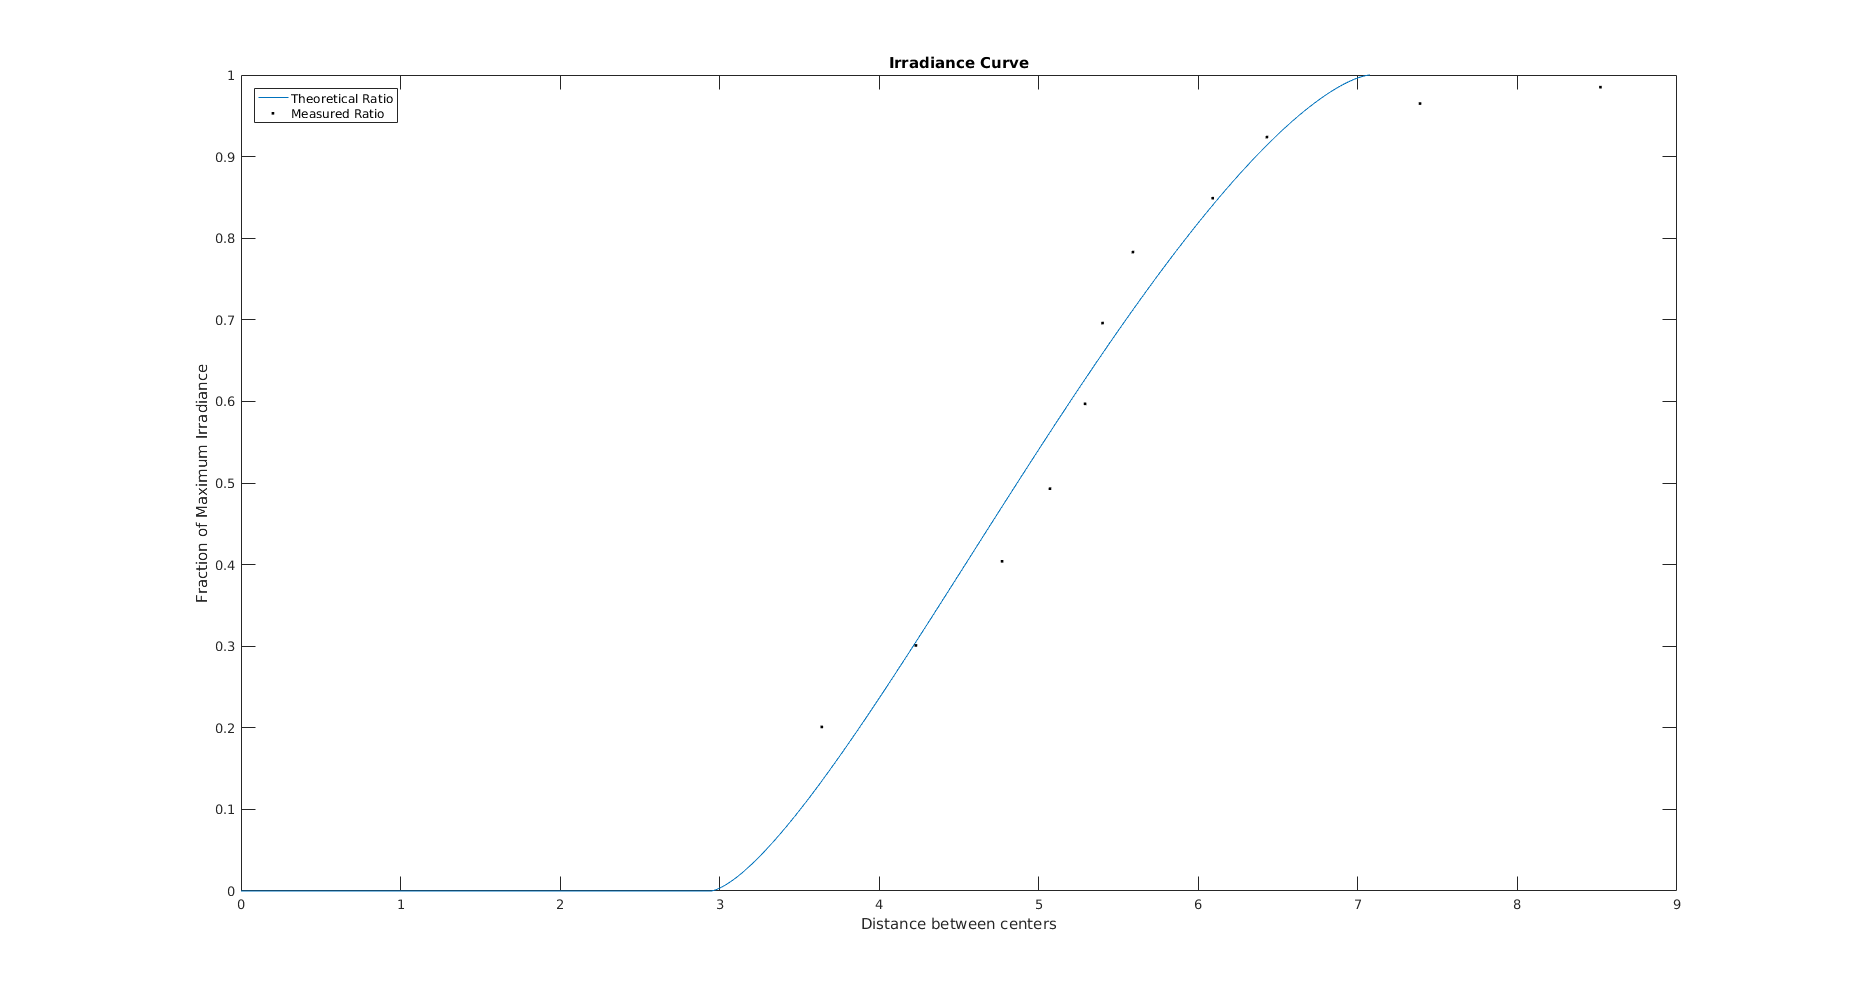
\includegraphics[scale=0.25]{parameterID/beam_block.png}
	\caption{Normalized Sensor Voltage Output vs Distance of Two Centers}
\end{figure}
Next, we will identify parameters of driver circuits. The resistance for driver circuits is given by
\begin{table}[H]
\begin{center}
    \begin{tabular}{|c|c|}
        \hline
        Component & Resistance ($\Omega$) \\ \hline
        $R_{1}$   & 44200                 \\ 
        $R_{2}$   & 984                   \\ 
        $R_{3}$   & 0.1                   \\
        \hline
    \end{tabular}
\caption{\emph{Measured Resistances in driver circuit.}}
\label{Q1_dt3}
\end{center}
\end{table}
Then we can calculate the theoretica relations between $I_{em}$ and $V_{in}$ which is:
$$I_{em}=\mf{1}{R_3}\left(\mf{R_2}{R_1+R_2}\right)V_{in} = \mf{1}{0.1 \,\Omega}\left(\mf{984 \,\Omega}{44.2 \,k\Omega + 984 \,\Omega}\right)V_{in} = 0.2177 \, V_{in}$$
We will use the experiment data measured with multimeter to compare with the theoretical curve shown as follows:
\begin{figure}[H]
	\centering
	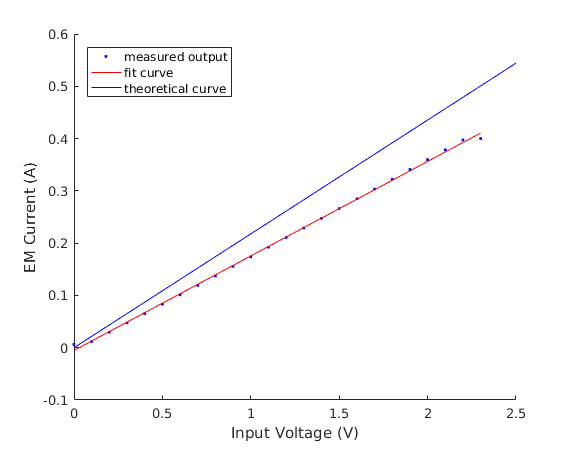
\includegraphics[scale=0.45]{parameterID/Driver_Circuit/dc_plot.png}
	\caption{Driver Circuit Current Voltage Relations}
\end{figure}	
The fit curve will have expression as:
$$I_{emfit} = 0.1808V_{in} - 0.005274$$
and we also observed that the current will get saturated to $400$ mA when $V_{in} > 2.3$ V.\\
Lastly, we need to identify parameters for electromagnetic force formula, which is $A$ and $B$. The nonlinear dynamic model for electromagnetic force is given in section (a).
$$F = f = \mf{AI^2}{B + x^2}$$
We first try to two sets of $\left(I,\; x\right)$ and use this two values to get the initial values for $A$ and $B$. In order to get the initial values for regression, we have to use following equilibrium equation to approximate:
$$mg = \frac{A I_{1}^2}{(B+x_{1})^2}  = \frac{A I_{2}^2}{(B+x_{2})^2}$$
Then we can transform it into a second order equation about $B$ and two sets of measured $\left(I,\; x\right)$ pair. That is
$$B^2(1-\mf{I_2^2}{I_1^2}) + (2x_1 - 2x_2\mf{I_2^2}{I_1^2})B + x_2^2 - x_1^2\mf{I_2^2}{I_1^2} = 0$$
If we choose $A = 1.9732\times 10^{-5}$ and $B = 0.0001998$, we will use a relatively good curve to fit the experiment data, the fitting plot is shown below:
\begin{figure}[H]
	\centering
	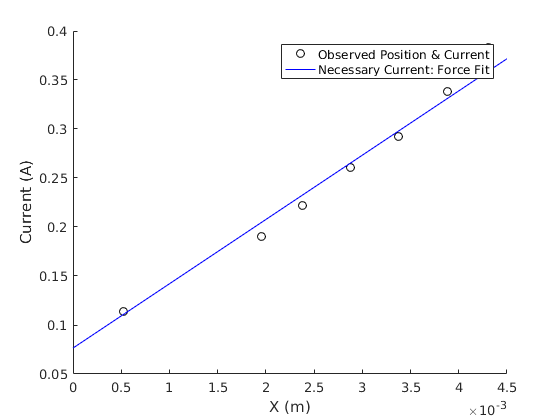
\includegraphics[scale=0.6]{parameterID/Magnet/current_position.png}
	\caption{Curve Fitting for Experimental data Current vs Position}
\end{figure}
We use methods above to get the parameters for physical system listed in the table below:
\begin{table}[H]
\begin{center}
    \begin{tabular}{|c|c|c|c|c|}
        \hline
        Mass & Nominal Equilibrium Point ($\bar{x}$) & Current at EQP ($\bar{i}$) & $A$ & $B$ \\ \hline
        $0.008$ kg   & $0.00321$ m & $0.046243$ A & $1.9732\times10^{-5}$ & $0.0001998$   \\ 
        \hline
    \end{tabular}
\caption{\emph{Identified Parameters for Physical System.}}
\label{Q1_dt5}
\end{center}
\end{table}
Substitute these parameters to the open loop transfer function we derived in part $\left(b\right)$, we get the numerical form shown below:
$$\mf{\hat{X}}{\hat{I}} = \mf{-1962}{s^2 - 26611.1}$$

\subsection*{(e)}
The Simulink model for nonlinear model is shown beolow:
\begin{figure}[H]
	\centering
	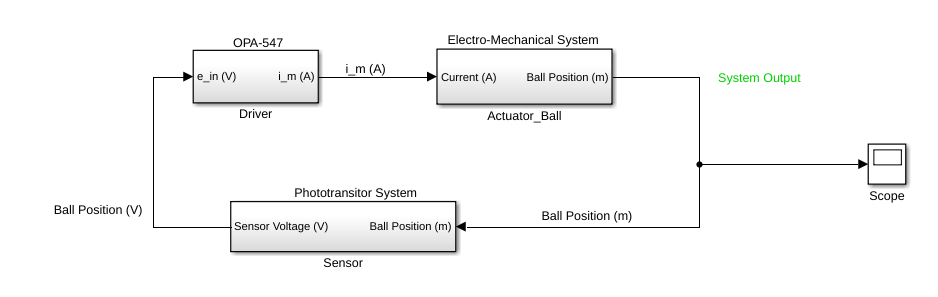
\includegraphics[scale=0.4]{nonlinear_open_loop.png}
	\caption{The overall open loop model for nonlinear system}
	\centering
	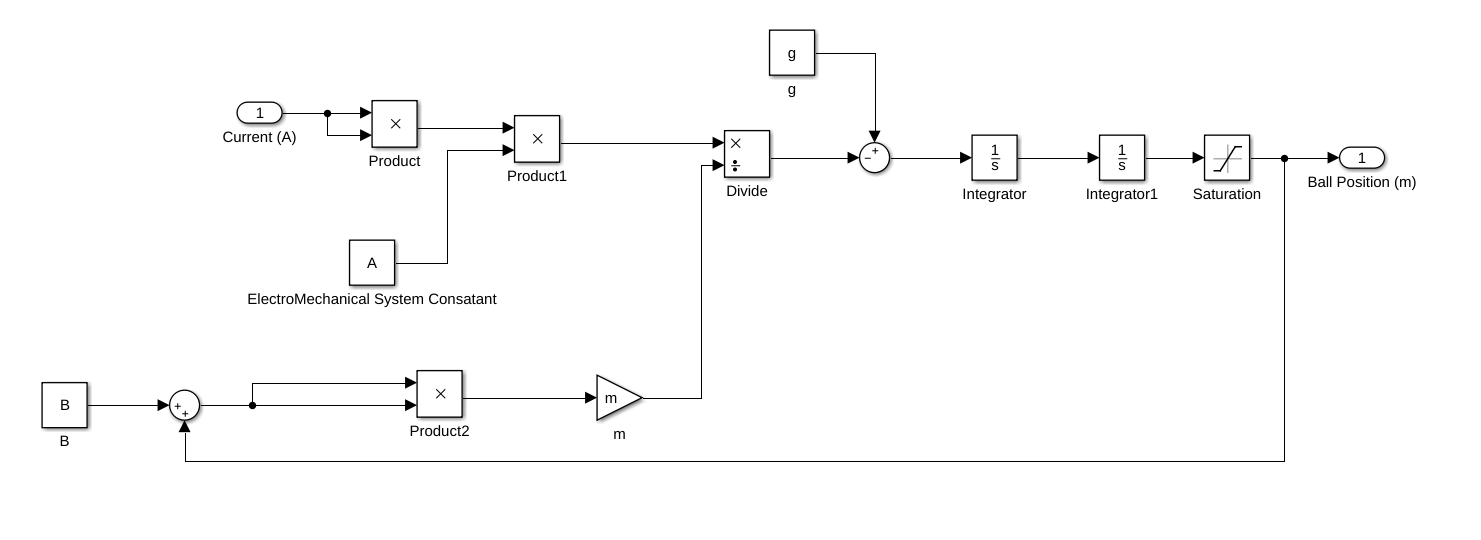
\includegraphics[scale=0.3]{nonlinear_actuator_ball.png}
	\caption{Subsystem for Actuator and Ball}
	\centering
	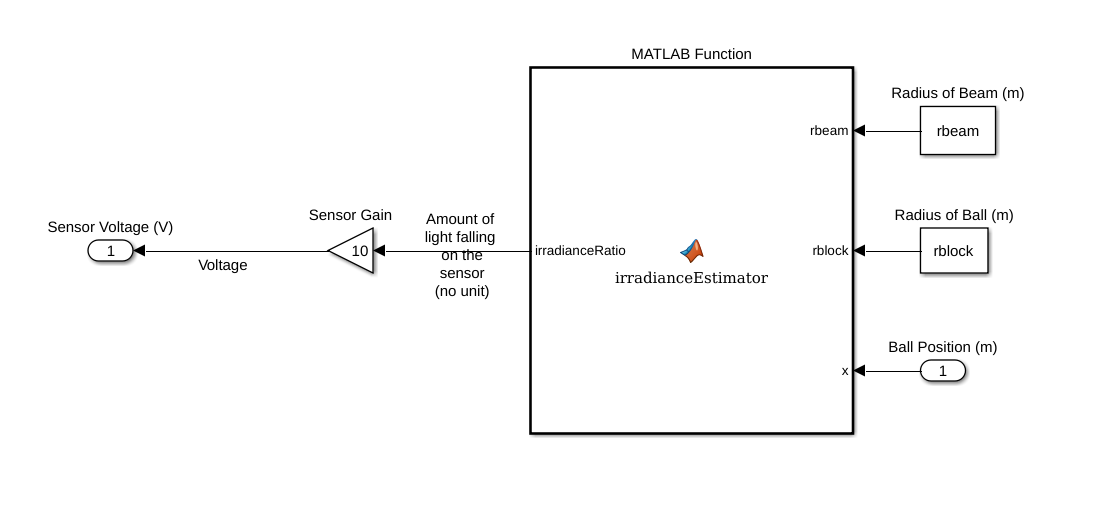
\includegraphics[scale=0.4]{nonlinear_sensor.png}
	\caption{Subsystem for Photo Transistor}
\end{figure}
Note here we use an irradiance Estimator module to calculate the light fraction received by the photo transistor, the values set to the parameter $rbeam$ and $rblock$ should be the optimal value we get from nonlinear regression using the experimental data.
\begin{figure}[H]
	\centering
	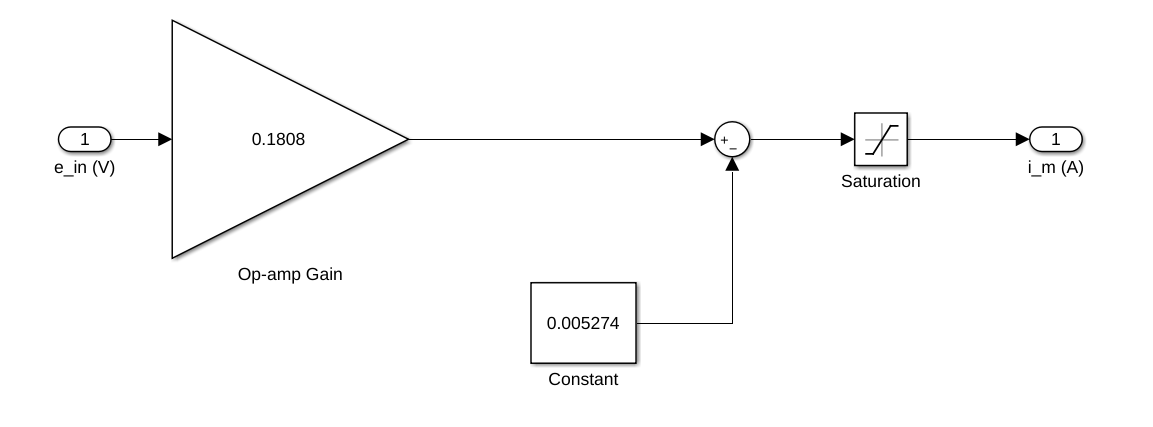
\includegraphics[scale=0.4]{nonlinear_driver_circuit.png}
	\caption{Subsystem for Driver Circuits}
\end{figure}
The Simulink model for linearized system is shown below:
\begin{figure}[H]
	\centering
	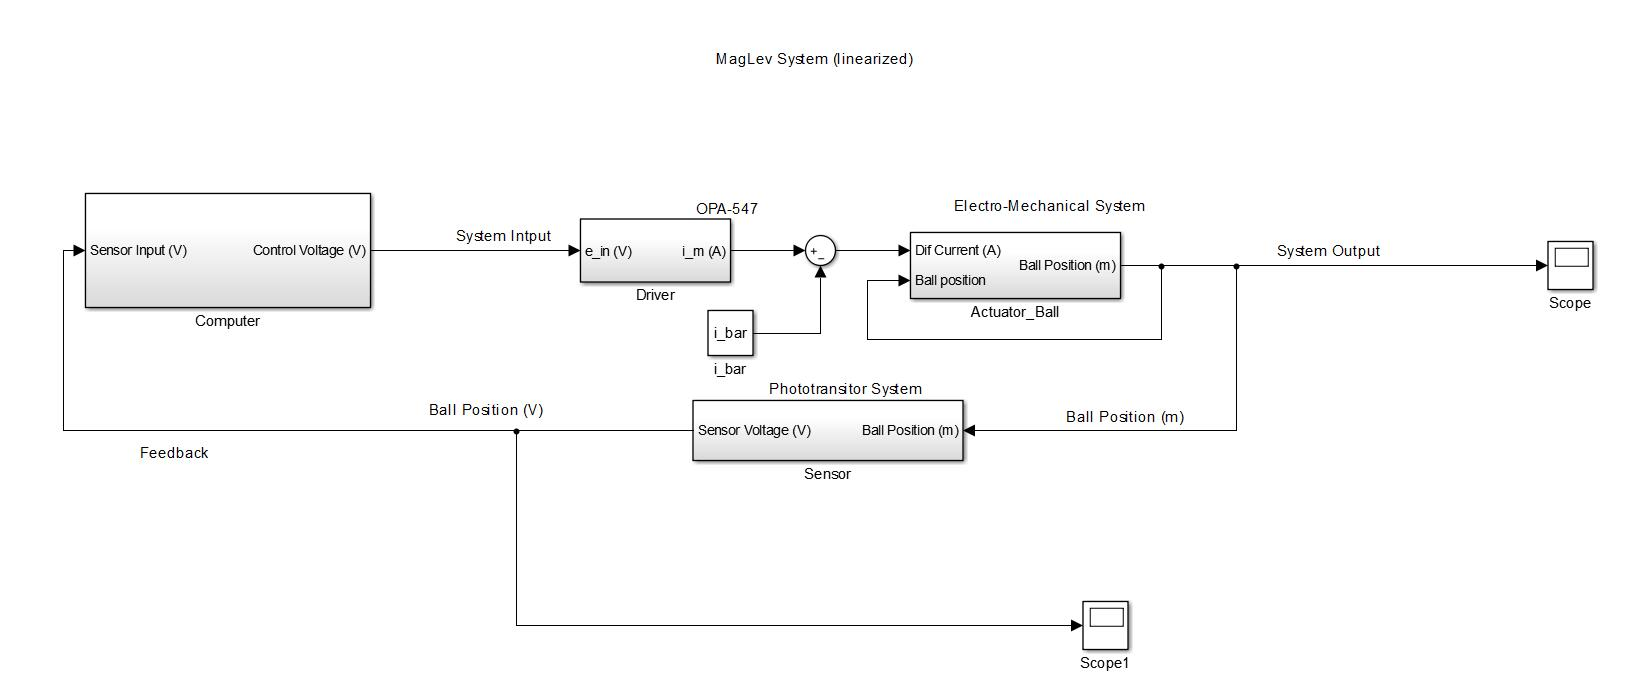
\includegraphics[scale=0.36]{Maglev system(linear).jpg}
	\caption{Linear Maglev System Model}
\end{figure}
The approximate linear model is shown below, we will use a first order polynomial to represent the relation.
\begin{figure}[H]
	\centering
	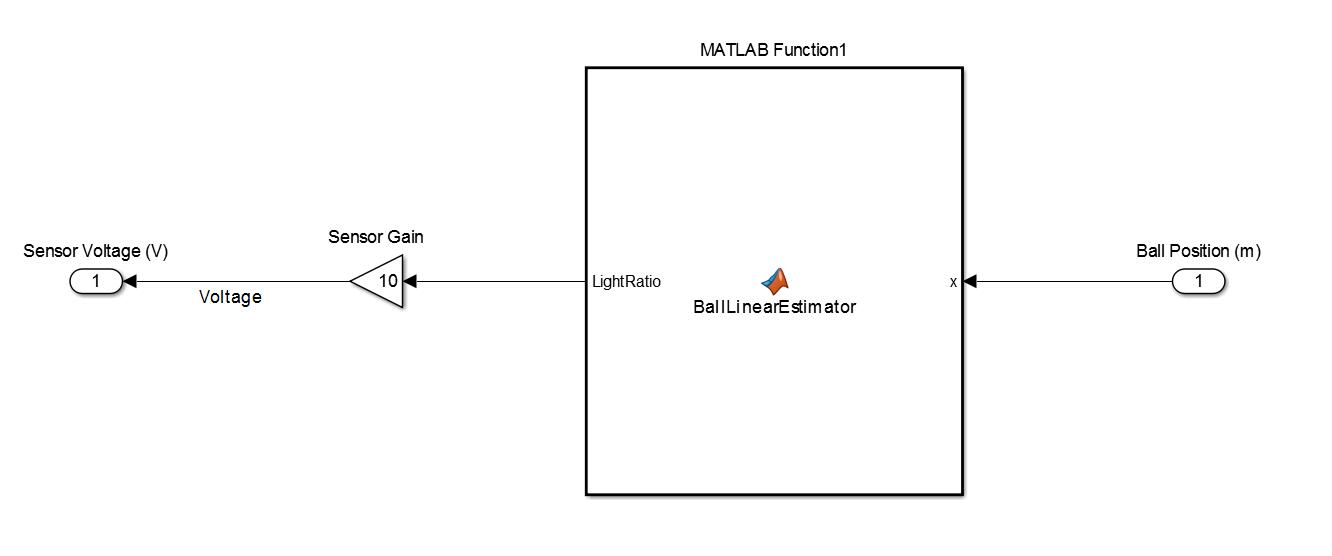
\includegraphics[scale=0.36]{sensor.jpg}
	\caption{Linear Model for Photo Transistor}
	\centering
	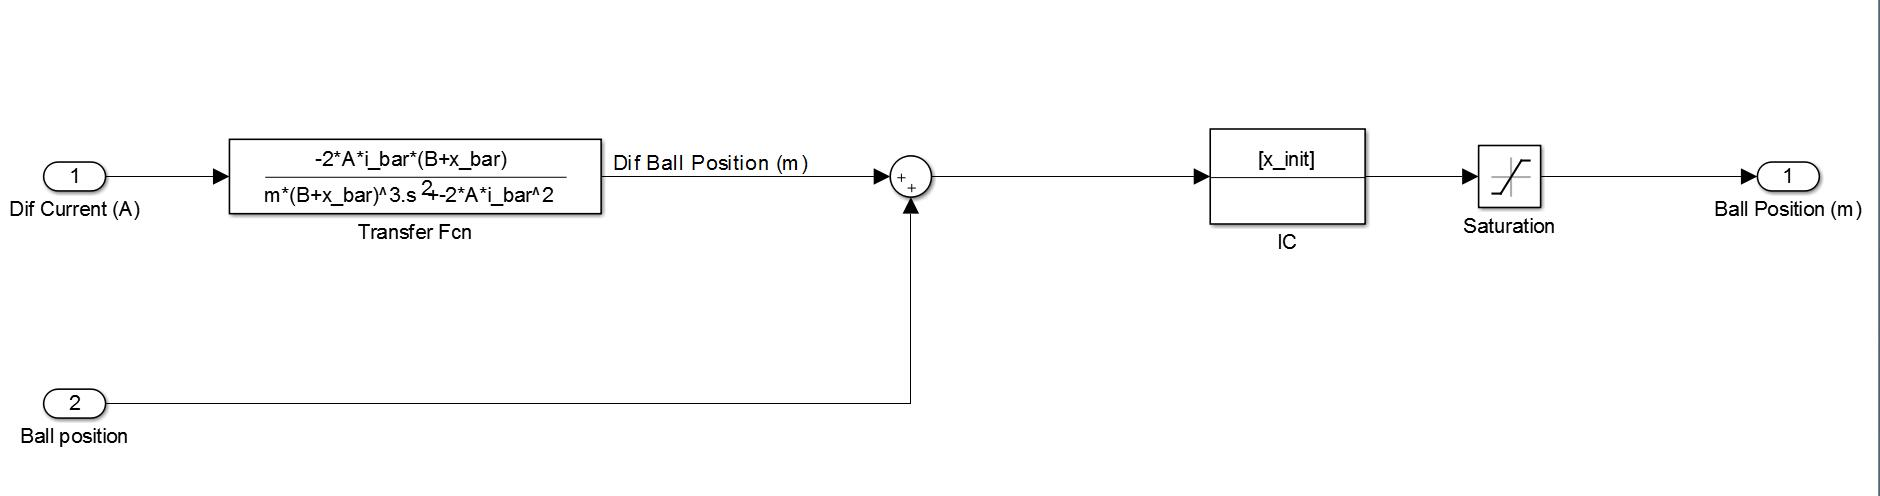
\includegraphics[scale=0.36]{Actuator_Ball.jpg}
	\caption{Linear Model for Dynamic System}
	\centering
	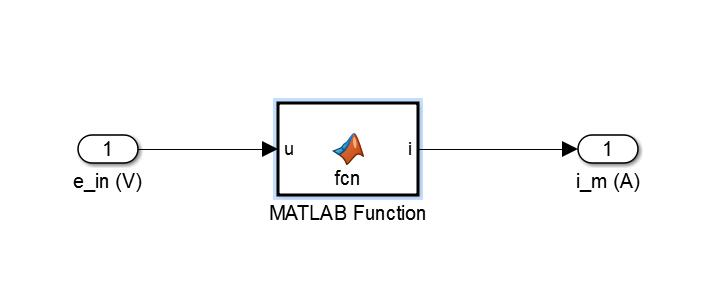
\includegraphics[scale=0.5]{Driver.jpg}
	\caption{Linear Model for Driver Circuits}
\end{figure}

\subsection*{(f)}
Now we will use the Simulink model to plot the uncontrolled system time response. We set the nominal initial position to be $\bar{x} = 0.00323 m$ and plot response in linear model and nonlinear model in the same graph:
\begin{figure}[H]
	\centering
	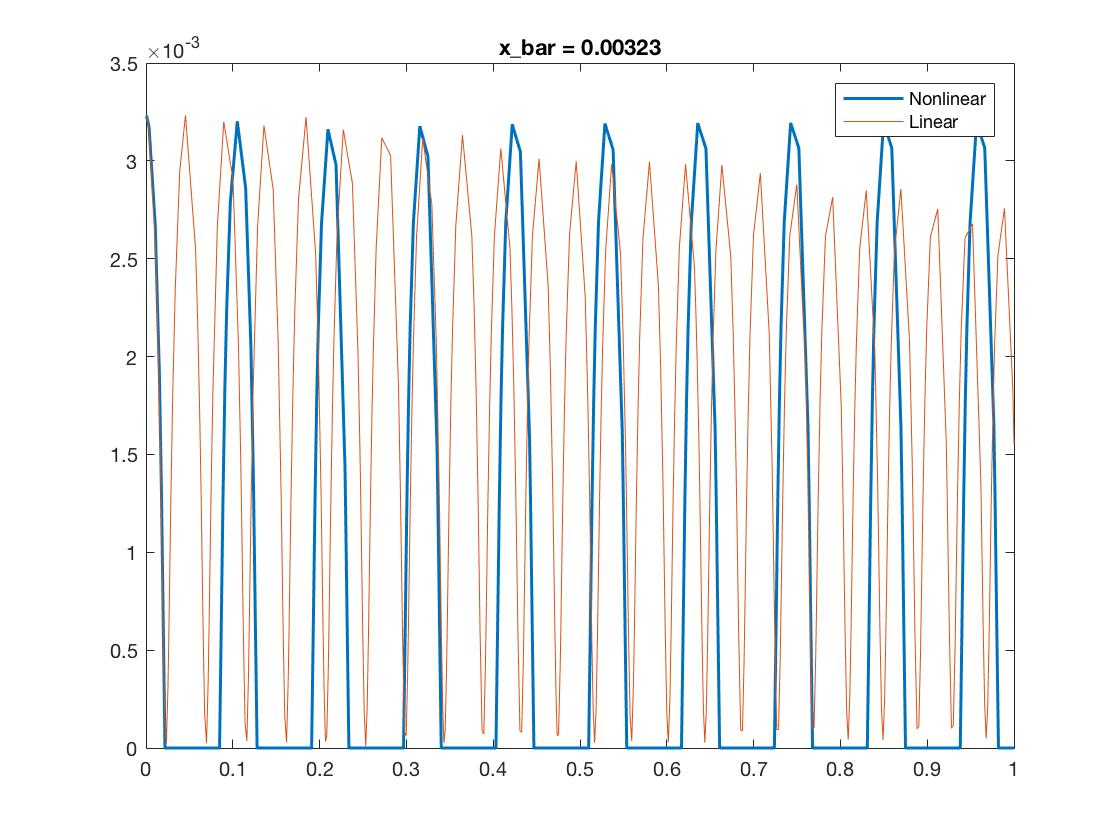
\includegraphics[scale=0.2]{X_BAR323_nocontrol.jpg}
	\caption{time response of linear and nonlinear sim model}
\end{figure}
We compare the time response plot of linear model and nonlinear model, we see the nonlinear model will oscillates more severely than linear model and it will collide with the end low surface of magnet, our linear model will predict a milder curve to oscillate around $1.9 mm$. Then we decide to take the initial position of the ball $0.01 mm$ closer to the magnet and see the changing trends of time response curves, we get the following results:
\begin{figure}[H]
	\centering
	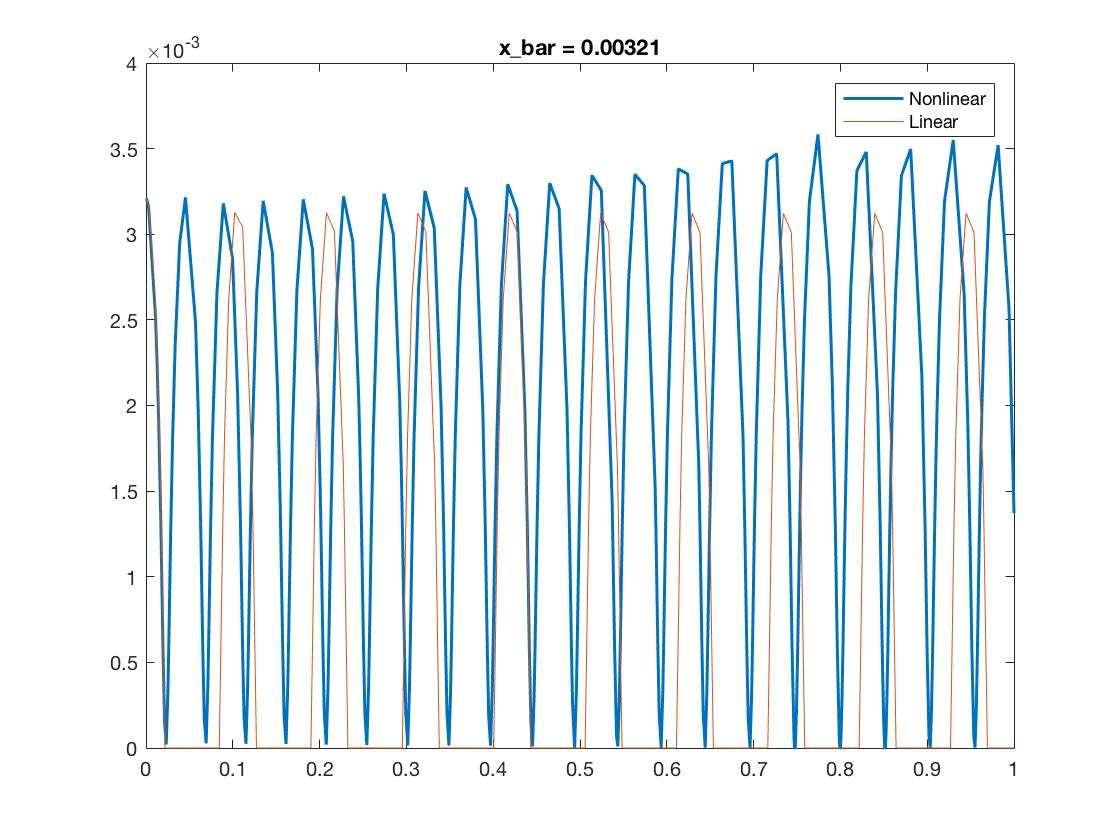
\includegraphics[scale=0.2]{X_BAR322_nocontrol.jpg}
	\caption{time response of linear and nonlinear sim model}
\end{figure}
In this case we see a similar trends as the previous case. At first, both of models will oscillate around the nominal initial position and a minimal distance point, then the nonlinear model will gradually oscillates more resonantly and the ball will become unstable to fall to ground. However, for linear model, the ball will oscillates for a few seconds and begin to slowly converge to a steady state, though for a small time step that may not be obvious. We think in the same condition the linear model will be more stable than nonlinear model since nonlinear model we need to consider the squared terms of current and displacement to formulate to dynamics which will render our system to behave more unpredicted when time grows. We think the real system if not added a controller will be unstable so that the nonlinear model may be more proper to describe the real system than linearized model.
\subsection*{(g)}
In order to test the fidelity of our linear model and nonlinear model, we could control some of our system parameters to be constant and change values of a specific parameter, use Labview and sensor to get the real time response and real time outputs of physical system. Compare them with the theoretical results and we can determine whether the linear model and nonlinear model is reasonable or not.
\section*{Question 2}
\subsection*{(a)}
We suppose to add a lead controller to the system. From the open loop transfer function we know the system is unstable, we can add a lead controller to our system to increase the phase margin, in order to compensate the decrease of gain margin, we also need to add a pole which is greater to zero to the controller transfer function so that we can increase the gain margin at a higher frequency point. Actually, our lead controller is not an ideal lead controller, since the transfer function will have a pole to play a role as phase lag. Using SISOTOOL in matlab, we can drag the zeros and poles of controller transfer function so that the poles and zeros of the overall closed loop transfer function can also changed. When all the poles of the closed loop transfer function lies on the left hand side of root locus plot, we will have a stable closed loop system. After configuring sisotool, we decide to set the transfer function for our linearized system as:
$$C(s) = \mf{-2000\left(1+0.0033s\right)}{\left(1+0.00056s\right)}$$
The loop transfer function for the overall system is:
$$L = \mf{-1962}{s^2 - 26611.1}\cdot\mf{-2000\left(1+0.0033s\right)}{\left(1+0.00056s\right)}$$
and closed loop transfer function is $\tfrac{L}{1+L}$. The closed loop bode plot is shown below:
\begin{figure}[H]
	\centering
	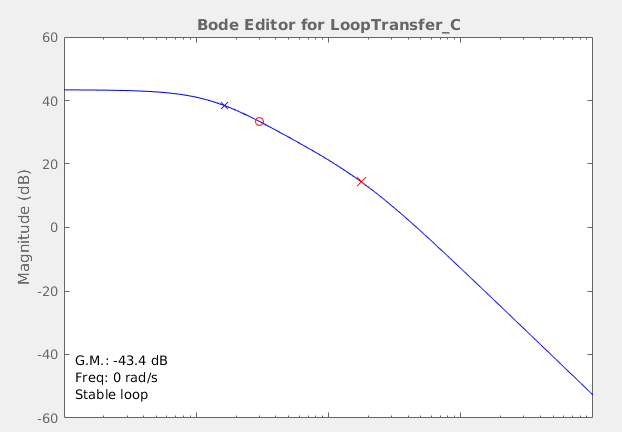
\includegraphics[scale=0.5]{bode_gain.png}
	\caption{Bode Plot of Loop Transfer Function}
\end{figure}
The bandwidth of the system is the frequency at which the gain of loop transfer function decreases to $3 dB$, in this case it is $4 \times 10^3 rad\cdot s^{-1}$. The root locus plot for loop transfer function is plotted.
\begin{figure}[H]
	\centering
	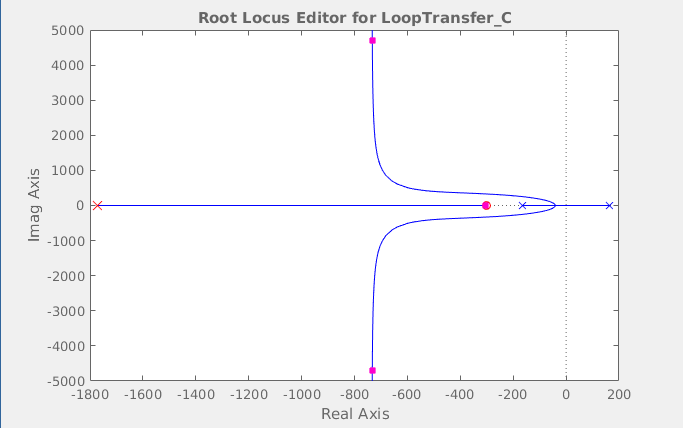
\includegraphics[scale=0.5]{root_locus.png}
	\caption{root locus plot of loop transfer function}
\end{figure}
\subsection*{(b)}
The linear and nonlinear Simulink model with controller added to them are shown before. We use the closed Simulink model to test experiments and get results shown in figures below:
\begin{figure}[H]
	\centering
	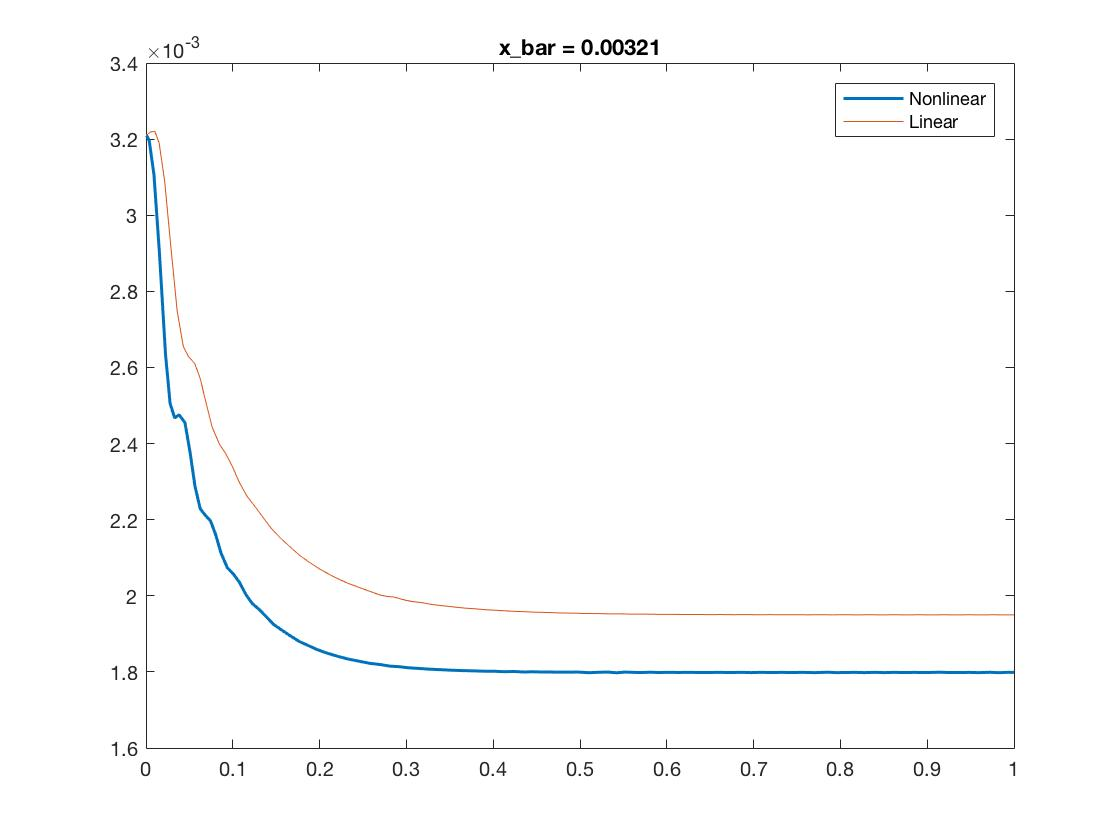
\includegraphics[scale=0.25]{X_BAR323_control.jpg}
	\caption{Closed Loop Time Response for $\bar{x} = 0.00321$}
\end{figure}
We see the linear and nonlinear models are both stable in this case and if we move the ball closer and closer to the magnet, we find the the controller will enforce the stability of our system but the robustness of linearized system will be better than nonlinear system in overall.
\subsection*{(c)}
The controller above does match the controller we used in the lab exercise during the previous week. Initially we had designed a new controller for this exercise, with different pole and zero locations, and a different gain value. However, both the nonlinear and linearized Simulink models were unstable under all of the conditions and variations we attempted. After discarding the new values and using the same poles, zeros, and gains that we had implemented in LabView on the test apparatus, the models became stable. This may be because prior to designing the controller for LabView, we conducted numerous tests to identify the parameters of the real system and modeled the various sub-systems. 
\subsection*{(d)}
The block diagram in figure nonlinear Simulink model illustrates how we ensure we have negative feedback in our system. If we start at the far right and assume that the ball just moved slightly above the set point (closer to the electromagnet), the sensor outputs a voltage related to this position which will always be positive. This voltage is then converted to position (m) and subtracted from the set point. Because the ball is above the set point, the error will be positive. The error signal then passes through a gain block of -1 to flip its sign to negative. The controller takes in the negative error and outputs a negative voltage. By adding this negative voltage to the bias voltage, a lower command voltage is sent to the driver than previously (the starting assumption was that the ball had been at the setpoint, but just moved up). This results in a smaller current being sent to the actuator, which results in less force from the electromagnet. Less force from the electromagnet results in the ball falling further away from the magnet, back towards the set point. This is the behavior that we want.

\section*{Question 3}
In our system, for the equilibrium point, the desired voltage is $V_{desire}=0.9 V$, bias voltage $V_{bias}= 1.85 V$. After experiment, we found that $V_{command}$ varies from $0.65V$ to $1.16V$. In our Simulink program, the non-linear model can range from $V_{command}= 0.16V$ to $1.49V$, while the linear model should be range from $0V$ to $1.52V$.\\
According to what’s above, controllable range of linear control system is larger than our experimental results, while the range is around the balanced position. As for nonlinear control system, the range is even larger and also ranged around the equilibrium point. Both models agreed on that the iron ball is controllable.\\
We think it is not likely to accurately predict the actual range in the experiment since some assumptions in modelling the system cannot apply in real life situations. For example:\\ 
1. For our driver circuits we assume the Op-Amp is ideal. Voltage at inverting and non-inverting terminals is equal and their current is zero. The input impedance is infinite and output impedance is zero.\\
2. For our feedback sensor system, we assume that when the path between the emitter and detector is completely blocked, no current flows through the detector. When no object is placed between the emitter and detector, a maximum amount of current flows through the detector. The current flowing through the transistor is converted to a voltage potential across a (sense) resistor. The light from the emitter are parallel to each other and they are not influenced by irrelevant objects in the neighborhood. \\
3.For our electromagnet system, we assume flux density is uniform for all cross section, and the material is linear in this system, etc.\\
4.Others assumptions like there is no air flow resistances, the heated electromagnet will not cause any side effects in our system, etc.\\
When we measured the system response, the input signal varies from 0.01Hz to 70Hz. The reason why we stop at 70Hz is that the labview program went into error when trying to collect data in 100Hz. The amplitude of the sinusoidal signal is about 0.048V and the experimental data(magnitude and phase) is attached below along with the ideal Bode plot(\ref{fig:bode}).
From the picture above, we noticed that no significant difference can be found on the Bode amplitude curves. The amplitude of the experimental Bode plot is almost as predictable at lower frequency such as those below 5Hz. The measurement runs into unstable situations when the phase curve approaches its phase margin. Fortunately, the tendency of amplitude is acceptable.
On the other hand, the phase curve is larger than we expected, in the lower frequencies, deference between ideal value and the experimental value is about $10^{\circ}$ to $20^{\circ}$, and phases keep shifting on higher frequencies, such as 7Hz and more. These errors may result from the non-linear fragments of the Meg-Lev system since we use the linearized model as the theoretical reference. Moreover, the magnitudes of noises are somehow proportional to the frequency of the sinusoidal signals. As the frequency grows, noises from the electrical circuit gains larger thus cause the phase measurement even more inaccurate.
\begin{figure}[H]
	\centering
	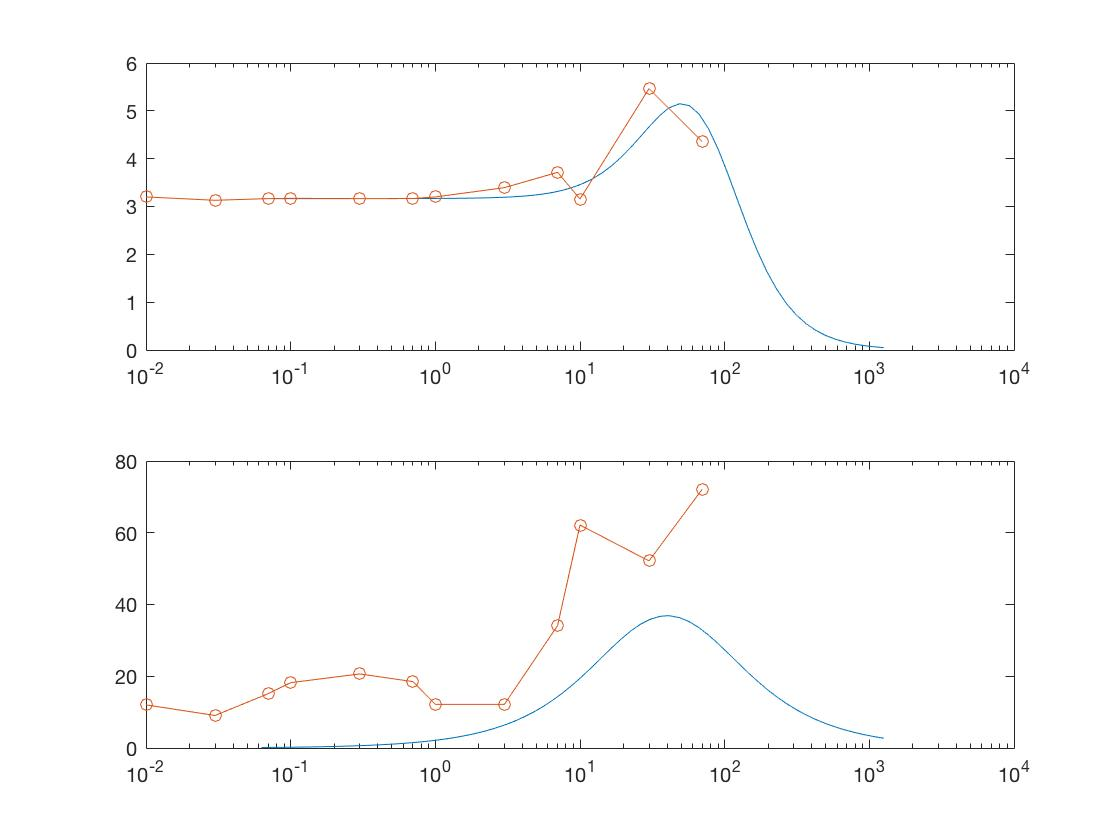
\includegraphics[scale=0.36]{bode.jpg}
	\caption{The Approximate Bode Plot vs Theoretical Bode Plot}
	\caption{fig:bode}
\end{figure}
\end{document}
